\chapter{DESAIN DAN IMPLEMENTASI}
\label{chap:desainimplementasi}

% Ubah bagian-bagian berikut dengan isi dari desain dan implementasi
Penelitian ini dilaksanakan sesuai dengan desain sistem berikut dengan implementasinya. Desain sistem merupakan konsep dari pembuatan dan perancangan infrastruktur dan kemudian diwujudkan dalam bentuk blok-blok alur yang harus dikerjakan. Sedangkan untuk bagian implementasi merupakan pelaksanaan teknis untuk setiap blok pada desain sistem.

\begin{figure}[h!]
  \begin{center}
    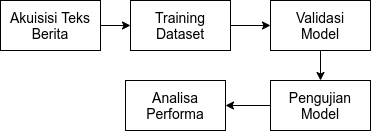
\includegraphics[width= 0.7\linewidth]{gambar/research_flow.png}
    \caption{bagan umum metodologi penelitian}
    \label{fig: base_method}
  \end{center}
\end{figure}

Gambar \ref{fig: base_method} merupakan bagan yang menunjukkan secara garis besar bagaimana proses implementasi model pada penelitian ini. Proses \textit{training} akan dilakukan beberapa kali dengan merubah parameter dari model untuk meningkatkan tingkat akurasi pada model akhir.

\section{Desain Sistem}

Tugas akhir ini adalah penelitian dalam bidang pemrosesan teks yang bertujuan untuk mendeteksi suatu berita hoaks berbahasa Indonesia secara otomatis berbasis \textit{Deep Learning}. Dalam proses \textit{training}-nya model ini akan menggunakan data yang dikumpulkan dari situs - situs berita yang sudah terverifikasi dan situs berita yang memang berisi berita palsu yang sudah ditemukan.


\section{Alur Kerja}

Terdapat beberapa langkah dalam melakukan implementasi dalam penelitian ini. Tahapan - tahapan ini sesuai berdasarkan dengan metodologi penelitian, yaitu :

\begin{enumerate}[nolistsep]
  \item Akuisisi Data
  \item \textit{Pre-Processing}
  \item Proses \textit{Training}
  \item Proses Pengujian
  \item Analisa Performa
\end{enumerate}

Berdasarkan bagan pada gambar \ref{fig: base_method}, proses yang pertama kali dilakukan adalah proses akuisisi data. Data yang diambil adalah data berupa berita yang berasal dari situs yang sudah terverifikasi seperti \url{liputan6.com}, \url{detik.com}, dan sebagainya. Selain itu, kami juga mengambil data berupa berita palsu yang sudah dipastikan sebagai palsu yang berasal dari situs seperti \url{turnbackhoax.com}. Tujuan dari proses akuisisi data ini adalah karena hampir tidak ada set data yang cukup banyak yang dapat digunakan sebagai data untuk proses klasifikasi berita palsu. Pada proses akuisisi ini juga dilakukan proses memberi label kepada kumpulan data dengan melihat tautan sumber berita.

Setelah set data berhasil didapatkan, proses selanjutnya adalah \textit{training} dimana data akan dimasukkan ke dalam model yang menggunakan metode berbasis \textit{Transformer} yaitu \textit{\textbf{B}idirectional \textbf{E}ncode \textbf{R}epresentations from \textbf{T}ransformers}(BERT).

\section{Akuisisi Data}

Pada tahap akuisisi data, data diambil dari situs - situs berita berbahasa Indonesia yang beredar di internet. Data - data tersebut akan diambil menggunakan metode \textit{webcrawling} sehingga diharapkan, apabila suatu saat diperlukan data dengan jumlah yang lebih banyak dapat dengan mudah memanggil program \textit{webcrawling} yang sudah dibuat. Untuk saat ini, keseluruhan kode program dapat diakses dan diunduh pada tautan \url{https://github.com/chillytaka/berita-crawler}.

\subsection{Sumber Akuisisi Data}

Sebagai dasar awal dari dataset, kami menggunakan dataset yang bersumber dari situs \url{https://data.mendeley.com/datasets/p3hfgr5j3m/1}. Namun, karena jumlah data dari situs tersebut dinilai kurang memadai untuk penelitian ini (data dari sumber tersebut hanya berjumlah 600 data), kami memutuskan untuk menambah dataset lagi menggunakan teknologi \textit{webcrawling}.

Sumber data yang pertama diambil berasal dari beberapa situs berita yang sudah terverifikasi seperti \url{liputan6.com}, \url{detik.com}, \url{kompas.com}, \url{cnnindonesia.com}. Sumber - sumber berita terverifikasi ini dipilih untuk menghilangkan proses pemberian label setelah dataset terkumpul. Diharapkan dengan mengambil teks berita dari situs yang sudah terpercaya dapat membuat model mengetahui bagaimana teks suatu berita yang berasal dari sumber terverifikasi. Selain itu, untuk lebih mengerucutkan lagi, kami hanya mengambil berita yang membahas isu nasional dan tidak mengambil berita yang membahas olahraga, opini, maupun jenis tipe berita lainnya. Gambar \ref{fig: news_source} menunjukkan salah satu situs berita yang digunakan dalam pengambilan dataset penelitian ini.

\begin{figure}[h!]
  \begin{center}
    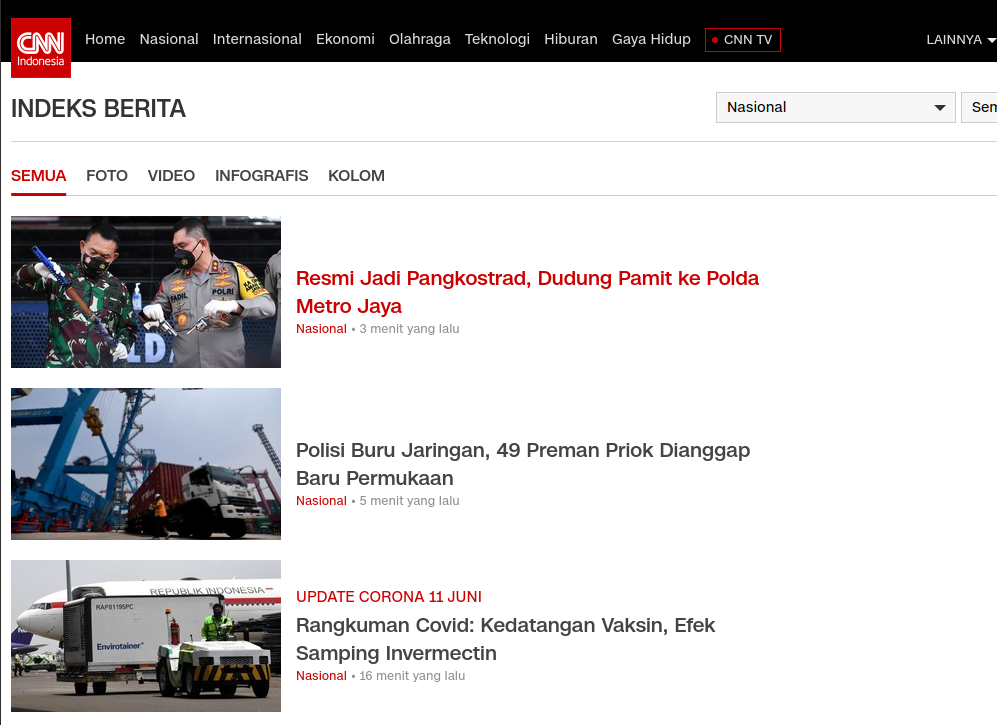
\includegraphics[width= .9\linewidth]{gambar/cnn_news.png}
    \caption{contoh situs sumber berita terverifikasi}
    \label{fig: news_source}
  \end{center}
\end{figure}

Sedangkan sumber kedua yang digunakan untuk proses pengambilan data pada penelitian ini adalah situs \url{turnbackhoax.id}. Situs tersebut adalah situs khusus yang mengumpulkan berita - berita yang sudah dipastikan palsu yang berasal dari berbagai sumber. Selain itu, situs ini juga mengambil data dari hasil unggahan masyarakat Indonesia sendiri melalui sosial media dan grup resmi \url{turnbackhoax.id}. Keuntungan dari metode seperti ini adalah sebuah unggahan akan dicek berkali - kali oleh anggota grup sehingga mengurangi kemungkinan terdapat berita yang salah klasifikasi. Alasan lain situs ini dipilih sebagai sumber adalah adanya format yang kurang lebih sama antara setiap unggahan sehingga akan memudahkan dalam proses pengambilan teks berita.

\begin{figure}[h!]
  \begin{center}
    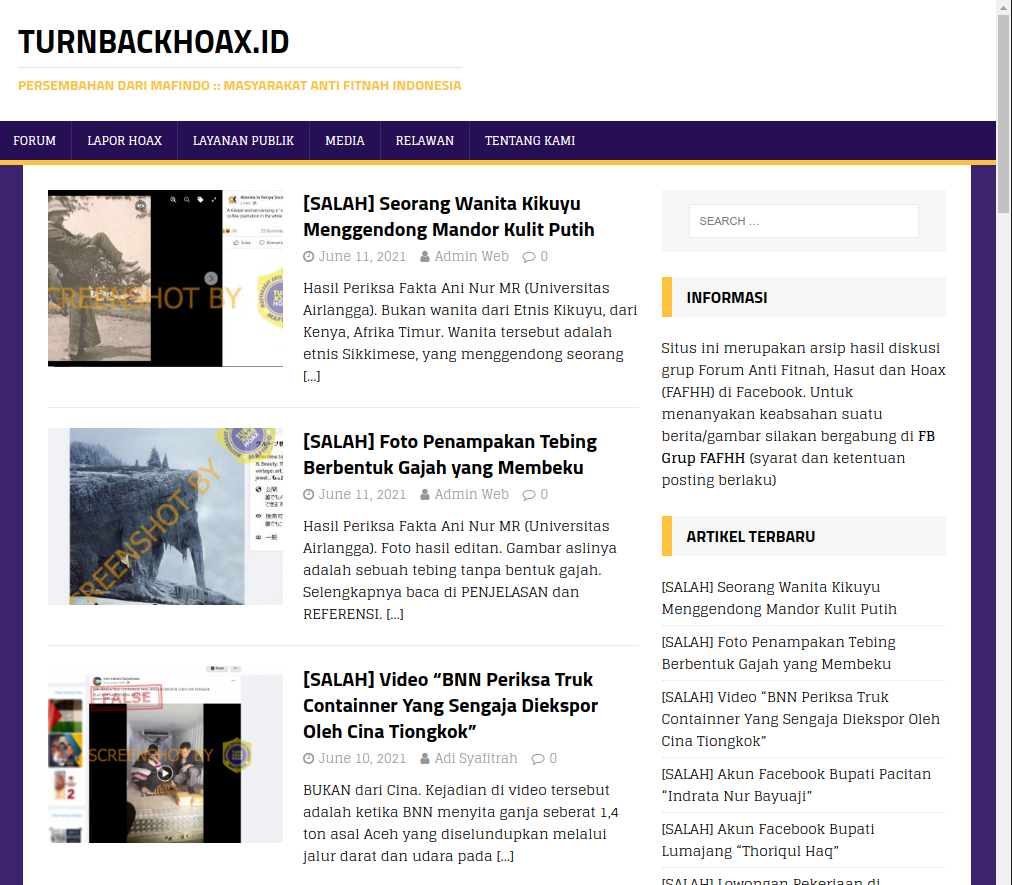
\includegraphics[width= \linewidth]{gambar/hoax_news.png}
    \caption{contoh situs sumber berita palsu}
    \label{fig: hoax_news_source}
  \end{center}
\end{figure}

\subsection{Proses Akuisisi Data}

Setelah menentukan situs - situs untuk digunakan sebagai sumber berita, langkah selanjutnya adalah memulai proses akuisisi data. Disini, hal yang paling pertama kali dilakukan adalah mengambil kode sumber dari situs - situs tersebut. Hal ini dilakukan guna mempermudah saat melakukan penyaringan untuk mendapatkan teks berita. Gambar \ref{fig:webcrawl_method} adalah gambaran garis besar yang kami lakukan dalam program \textit{web crawl} kami. Dimulai dengan memasukkan kode HTML mentah, kemudian merubah kode mentah tersebut menjadi objek yang lebih mudah untuk dilakukan pemrosesan dalam python, mengambil teks berita dan melakukan pembersihan terhadap teks tersebut, terakhir menghasilkan keluaran berupa file .CSV dengan format yang sesuai.

\begin{figure} [ht]
  \centering
  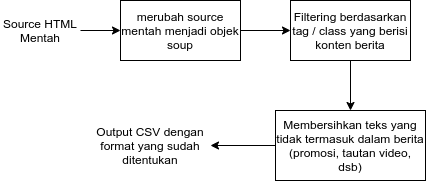
\includegraphics[width=.9\linewidth]{gambar/webcrawl method_box.png}
  \caption{Garis besar alur program \textit{web crawl}.}
  \label{fig:webcrawl_method}
\end{figure}

\begin{figure}[h!]
  \begin{lstlisting}[
    language=HTML, 
    caption={Penggalan Kode Sumber HTML \url{detik.com}.},
    label={lst:source_detik}
]

...
<div class="detail__body itp_bodycontent_wrapper">
<div class="detail__body-text itp_bodycontent">

<strong>Jakarta</strong> - Koalisi <a href="https://
detik.com/tag/jokowi" target="_blank">Jokowi</a> 
sedang menyusun visi-misi jagoannya. Setelah 
menerima masukan dari <a href="https://detik.com/
tag/muhammadiyah" target="_blank"> Muhammadiyah</a>,
 ... 
Dan kita pun membuka diri untuk menerima 
masukan untuk penyempurnaan," imbuhnya.<br><br><!--
s:parallaxindetail--><div class="clearfix"></div><style>
...

\end{lstlisting}
\end{figure}

\textit{Library} yang kami gunakan untuk melakukan \textit{crawling} adalah \textit{BeautifulSoup}, sebuah \textit{library} yang akan secara otomatis merubah dari suatu teks HTML menjadi objek \textit{soup} yang lebih mudah untuk dilakukan pemrosesan di dalam python.

Yang pertama kali harus kami lakukan adalah menentukan \textit{tag} atau \textit{class} HTML yang akan digunakan sebagai masukan pada program guna melakukan penyaringan terlebih dahulu. Apabila merujuk pada listing \ref{lst:source_detik} \textit{class} yang berisi teks seluruh berita adalah \texttt{detail\_\_body\-text} sehingga kami melakukan penyaringan dengan memasukkan \textit{class} tersebut ke dalam parameter.

Namun, walaupun sudah melakukan penyaringan, masih terdapat beberapa teks yang tidak diperlukan. Biasanya, teks - teks tersebut masuk ke dalam  kategori seperti catatan dari penulis, iklan, dan tautan untuk menuju ke berita yang masih berhubungan. Sehingga, setelah melakukan penyaringan, masih diperlukan lagi pembersihan isi berita dari teks - teks yang tidak diperlukan.

Terakhir, adalah melakukan keluaran berupa \textit{file} .CSV. Alasan menggunakan format CSV sebagai keluaran adalah karena format tersebut bersifat 'terbuka' dan dapat dibuka oleh berbagai \textit{software} spreadsheet pada umumnya, selain itu akan lebih mudah memproses data dalam bentuk .CSV di python dibandingkan dengan format lainnya.

Untuk memudahkan penggunaan perangkat lunak \textit{webcrawler} yang kami buat, kami menggunakan berkas dengan format .json untuk mengatur sumber, banyak berita dan filter tanggal yang nantinya akan dibaca oleh program dan mengambil berita dengan parameter tersebut. Tabel \ref{tab:contoh_dataset} merupakan contoh hasil keluaran dari program \textit{webcrawling} yang digunakan.

\begin{table}
  \caption{Contoh Dataset}
  \label{tab:contoh_dataset}
  \centering
  \begin{tabular}{ | p{.7\linewidth} | l | }
    \hline
    \textbf{berita}                                                                                                                                                                                                                   & \textbf{\textit{tagging}} \\ \hline
    Wakil Gubernur DKI Jakarta Sandiaga Uno menargetkan pengerjaan tahap awal Stadion BMW dilakukan pada Oktober. Stadion ini diperuntukkan bagi klub Persija....                                                                     & Valid                     \\ \hline
    "Komisi II bersama KPU dan Bawaslu masih membahas ketentuan wajib cuti bagi petahana presiden yang maju Pilpres 2019. Mekanisme pengambilan.....                                                                                  & Valid                     \\ \hline
    Jaksa penuntut Ulumum (JPU) pada Komisi Pemberantasan Korupsi (KPK) mencecar Pejabat Pembuat Komitmen (PPK) reguler pada Direktorat Perlindungan Sosial Korban Bencana Sosial Kemensos Victorious Saut Hamonangan Siahaan soal... & Valid                     \\ \hline
    “Halo Kak! Aku Winda Dari Team Giveaway BAIM WONG Anda Memenangkan Hadiah Uang 100Jt dari kami info klik: https://wa.me/+6285796306857”                                                                                           & Hoax                      \\ \hline
    “Apa yang terjadi dengan hewan dalam penelitian?   Teknologi ini telah dicoba pada hewan, dan pada hewan penelitian yang dilakukan, semua hewan mati , tidak langsung dari suntikan...                                            & Hoax                      \\ \hline
    “Kadrun istilah dr PKI alias KOMUNIS ditujukan buat islam. Kl mau jd komunis pake aja istilah kadrun buat umat islam. Auto lsg Komunis”                                                                                           & Hoax                      \\ \hline
  \end{tabular}
\end{table}

Setelah melakukan penggabungan antara data yang berasal dari \url{https://data.mendeley.com/datasets/p3hfgr5j3m/1} dengan dataset hasil dari proses \textit{webcrawling}, maka didapatkan total data sebesar 1621 data dengan pola penyebaran data yang kurang lebih seimbang sehingga mengurangi kemungkinan terjadinya bias pada saat proses melatih model. Tabel \ref{tab:dataset} menunjukkan secara lebih detail berapa banyak distribusi  data yang berada di dalam dataset yang digunakan dalam penelitian ini.

\begin{table}
  \caption{Jumlah Dataset yang digunakan}
  \label{tab:dataset}
  \centering
  \begin{tabular}{ | l | l | }
    \hline
    \textbf{Label} & \textbf{Jumlah Data} \\ \hline
    \textit{Hoaks} & 885                  \\ \hline
    \textit{Valid} & 736                  \\ \hline
    \textbf{Total} & \textbf{1621}        \\ \hline
  \end{tabular}
\end{table}

\section{\textit{Preprocessing}}

\begin{figure}[h!]
  \begin{center}
    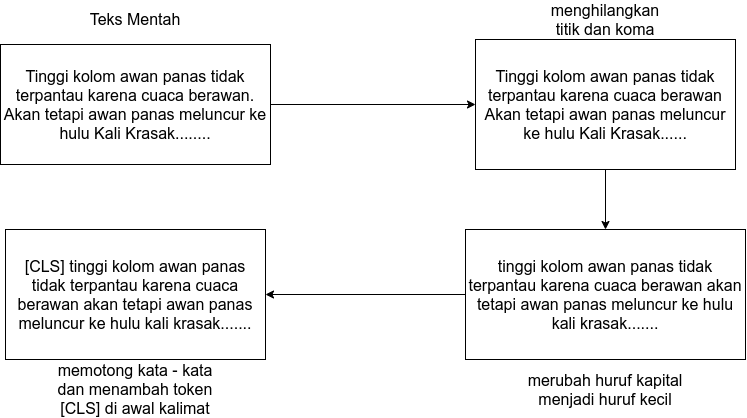
\includegraphics[width= \linewidth]{gambar/preprocess.png}
    \caption{Metode Preprocessing}
    \label{fig: metodologi_preprocessing}
  \end{center}
\end{figure}

Pada proses ini, data akan disiapkan terlebih dahulu agar dapat diproses oleh BERT. Proses penyiapan data meliputi menghilangkan titik dan koma, dan merubah huruf kapital yang ada menjadi huruf kecil seluruhnya. Dan karena BERT memiliki maksimal kata - kata yang dapat diproses dalam sekali waktu sejumlah 512 kata atau token, maka harus dilakukan penyingkatan teks, dapat dengan cara melakukan pengambilan 512 karakter pertama, terakhir maupun gabungan dari kedua bentuk. Chi Sun et al. menemukan bahwa mengambil teks dengan cara mengambil bagian tengah sebanyak 128 kata pertama dan mengambil sebanyak 382 kata pada bagian akhir menghasilkan hasil akurasi yang lebih baik dalam beberapa tugas \cite{sun2019fine}. Langkah terakhir adalah menambahkan token \texttt{[CLS]} di awal kalimat. Untuk lebih jelasnya, bisa melihat pada Gambar \ref{fig: metodologi_preprocessing}.

Selain itu, juga akan dilakukan pembagian dataset yang awalnya berjumlah 1621 akan dibagi menjadi 3 bagian dengan ketentuan 70\% akan digunakan pada saat proses \textit{training}, 10\% akan digunakan untuk proses validasi, dan sisanya sebesar 20\% akan digunakan pada saat pengujian.

\begin{enumerate}
  \item \textit{Training}

        Set ini digunakan oleh algoritma BERT sebagai masukan saat melakukan proses \textit{training} sehingga akan didapat model yang sesuai.

  \item Validasi

        Set ini digunakan pada saat selesai melakukan validasi model setelah melakukan \textit{training}. Digunakan untuk menentukan apakah suatu model sudah memiliki \textit{weight} yang sesuai ataukah masih perlu melakukan \textit{training} lagi. Selain itu, set ini juga digunakan untuk menghindari kemungkinan \textit{overfitting} maupun \textit{underfitting} dalam model.

  \item Pengujian

        Set yang digunakan untuk melakukan pengujian akurasi model setelah proses \textit{training} dan validasi selesai. Hasil akurasi dari pengujian inilah yang akan digunakan sebagai hasil dari model.

\end{enumerate}

Untuk lebih jelasnya, silahkan lihat tabel \ref{tab:dataset_section}. Dari tabel tersebut dapat dilihat bahwa pembagian dan total dari dataset sudah sesuai.

\begin{table}
  \caption{Rincian Pembagian Dataset}
  \label{tab:dataset_section}
  \centering
  \begin{tabular}{ | l | l | l | l | }
    \hline
    \textbf{Bagian}                      & \textbf{Hoaks} & \textbf{Valid} & \textbf{Total Data} \\ \hline
    \textit{Training}                    & 647            & 519            & 1166                \\ \hline
    \textit{Validasi}                    & 85             & 78             & 163                 \\ \hline
    \textit{Pegujian}                    & 153            & 139            & 292                 \\ \hline
    \multicolumn{3}{|l|}{\textbf{Total}} & \textbf{1621}                                         \\ \hline
  \end{tabular}
\end{table}

\section {Proses \textit{Training}}

\begin{figure}[h!]
  \begin{center}
    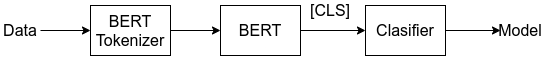
\includegraphics[width= 0.9\linewidth]{gambar/training.png}
    \caption{Metode Training}
    \label{fig: metodologi_training}
  \end{center}
\end{figure}

Pada tahap ini, teks yang sudah melewati proses \textit{preprocessing} akan dilakukan proses Tokenizer. Tokenizer adalah proses untuk merubah kata - kata dalam teks menjadi token sesuai dengan \textit{word embedding} yang sudah ada pada \textit{pretrained} BERT. Barulah pada saat itu, BERT dapat melakukan \textit{training} berdasarkan data dari \textit{dataset}.

Keluaran dari BERT akan diambil isi token \texttt{[CLS]}-nya dan dimasukkan kedalam algoritma klasifikasi, dalam penelitian ini kami memilih untuk menggunakan metode \textit{Linear Regression}. \textit{Linear Regression} digunakan sebagai algoritma klasifikasi yang cukup mudah namun memiliki tingkat akurasi yang cukup. Gambar \ref{fig: metodologi_training} dapat digunakan sebagai penjelas.

Pada tahap ini juga dilakukan pengaturan ukuran \textit{batch}, \textit{learning rate} dan juga \textit{epoch}. \textit{Batch} adalah banyaknya teks yang diproses untuk setiap iterasi, semakin tinggi nilai \textit{batch} yang dikonfigurasi, maka proses \textit{training} akan semakin cepat namun memakan memori yang lebih banyak. Berhubung algoritma BERT adalah algoritma yang cukup berat karena memiliki \textit{layer} yang cukup banyak, dan karena terdapat keterbatasan \textit{resource} maka dalam penelitian ini kami menggunakan \textit{batch} dengan nilai 8.

\textit{Epoch} adalah berapa banyak suatu algoritma melakukan proses \textit{training} dan validasi sebelum dianggap final. Disini \textit{epoch} harus diperhatikan agar jumlah \textit{loss} yang terjadi pada saat proses \textit{training} tidak terlalu tinggi karena merupakan ciri - ciri \textit{underfitting} namun juga tidak terlalu rendah selama beberapa \textit{epoch} untuk menghindari kemungkinan \textit{overfitting}. Berhubung kami hanya menggunakan BERT untuk memproses teks yang relatif lebih mudah, kami hanya menggunakan \textit{epoch} sebesar 10.

\textit{learning rate} adalah seberapa banyak \textit{hyperparameter} yang dirubah selama proses \textit{training}. \textit{hyperparameter} digunakan untuk merubah \textit{weight} selama proses \textit{training} berdasarkan \textit{feedback} saat proses validasi. Disini kami menggunakan nilai yang direkomendasikan oleh pembuat model BERT yang kami gunakan, yaitu 0.000002 \cite{koto2020indolem}.

\begin{table}
  \caption{Konfigurasi pada BERT}
  \label{tab:bert_config}
  \centering
  \begin{tabular}{ | l | l | }
    \hline
    \textbf{Jenis Konfigurasi} & \textbf{Keterangan} \\ \hline
    \textit{batch}             & 8                   \\ \hline
    \textit{learning rates}    & 2e-6                \\ \hline
    \textit{epoch}             & 5                   \\ \hline
  \end{tabular}
\end{table}


\section{Proses Pengujian}

Proses pengujian dalam penelitian ini dibagi menjadi 2 bagian, bagian yang pertama dilakukan pada saat model selesai melakukan proses \textit{training} namun masih memiliki iterasi \textit{epoch} yang belum selesai. Proses ini bernama validasi. Proses ini sangat vital karena dengan validasi kita dapat mengetahui apakah model kita mengalami \textit{overfitting} maupun \textit{underfitting}. Salah satu ciri yang paling mudah yang menandakan kemungkinan terjadinya \textit{overfitting} adalah ketika besaran \textit{training loss} suatu model menjadi semakin kecil, namun besaran \textit{validation loss}-nya malah semakin besar di setiap iterasi. Sedangkan \textit{underfitting} terjadi ketika baik \textit{training loss} maupun \textit{validation loss} memiliki nilai yang terlalu besar. Selain itu pada proses validasi ini, data yang digunakan adalah data yang sama sekali baru dan tidak digunakan selama proses \textit{training} guna menghindari kemungkinan terjadinya bias yang biasa terjadi apabila suatu model diuji pada data yang sama yang digunakan pada saat proses \textit{training}. Berdasarkan data pada proses validasi, algoritma \textit{optimizer} akan memutuskan untuk merubah \textit{weight} dalam \textit{hidden node} BERT sehingga semakin mendekati titk akurasi tertingginya.

Bagian selanjutnya dari proses pengujian adalah melakukan \textit{test}. Sama seperti pada waktu proses validasi, dataset yang digunakan juga sama sekali berbeda dengan data yang digunakan pada waktu \textit{training} maupun pada waktu \textit{validasi}. Dari proses ini, dapat diambil kesimpulan apakah suatu model tersebut dapat dilakukan perbaikan lagi denga cara \textit{re-training} dan merubah beberapa parameter maupun konfigurasi yang sudah diatur pada saat proses \textit{training}, ataukah model tersebut dirasa sudah cukup baik dan akan melanjutkan ke proses berikutnya.

\section{Analisa Performa}

Setelah melakukan proses pengujian, langkah berikutnya adalah melakukan analisa perforrma pada model yang sudah dibuat. Hal ini untuk mengetahui bagaimana kira - kira performa model pada saat sudah diimplementasi. Untuk analisa performa ini akan digunakan beberapa metode seperti \textit{confusion matrix} agar mendapat pengelompokkan berdasarkan data menjadi \textit{True Positive} (TP), \textit{False Positive} (FP), \textit{True Negative} (TN), dan \textit{False Negative} (FN). Selain itu, penelitian ini juga akan menggunakan rumus - rumus seperti \textit{Recall, Precision, F1-score}.

